\section{Einleitung}

Echtzeitsysteme müssen innerhalb genauer Zeitvorgaben auf Ereignisse in der Umgebung reagieren.
Sie sind; reaktiv, effizient, verläslich, betriebssicher, spezifisch und real-time.

\subsection{Rechenleistung}

\formula{$\mathit{Time} = \dfrac{\mathit{Seconds}}{\mathit{Program}} = \dfrac{\mathit{Instructions}}{\mathit{Program}} \cdot \dfrac{\mathit{Clock cycles}}{Instruction} \cdot \dfrac{\mathit{Seconds}}{\mathit{Clock cycle}}$}

\subsection{Sense-Think-Act Paradigma}

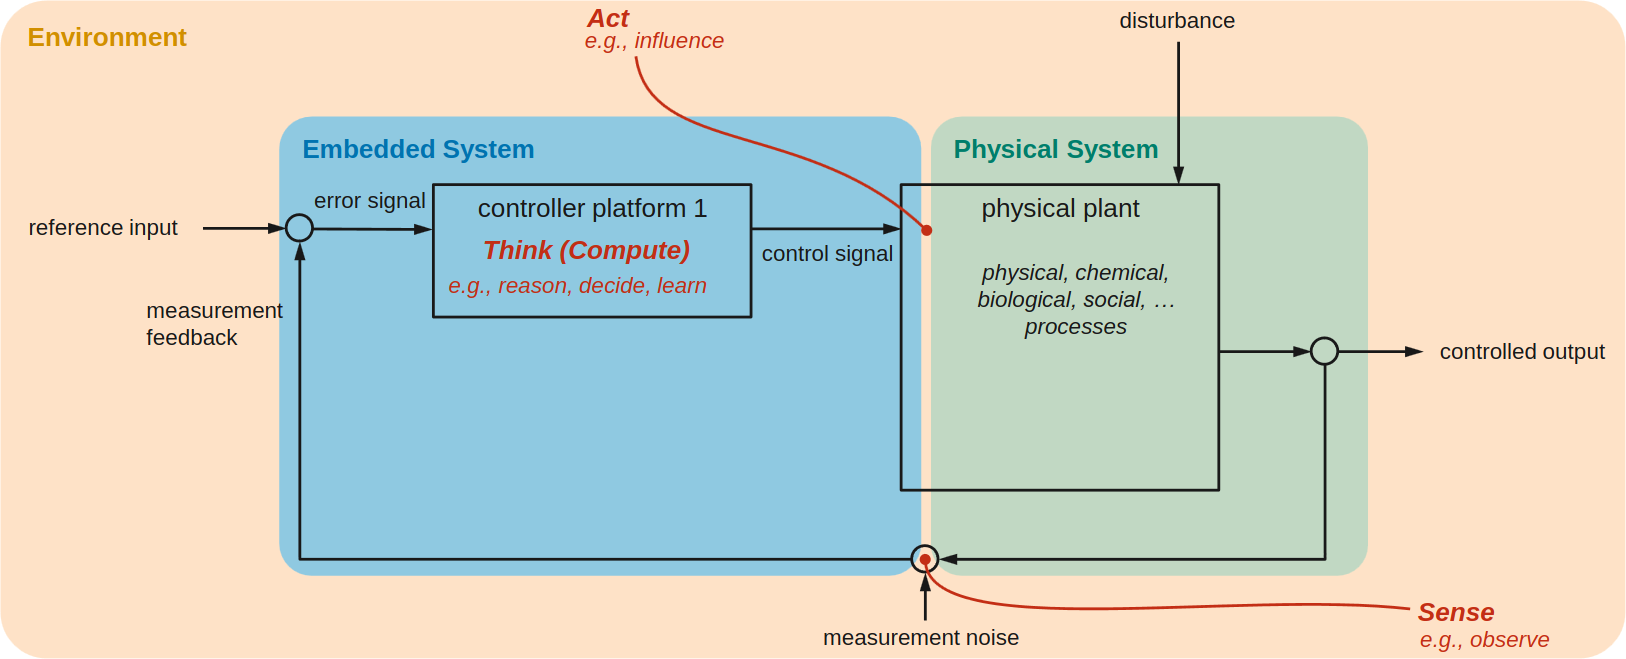
\includegraphics[width=\linewidth]{"Images/SenseThinkAct.png"}

Bei einem CPC (Cyber Physical System):

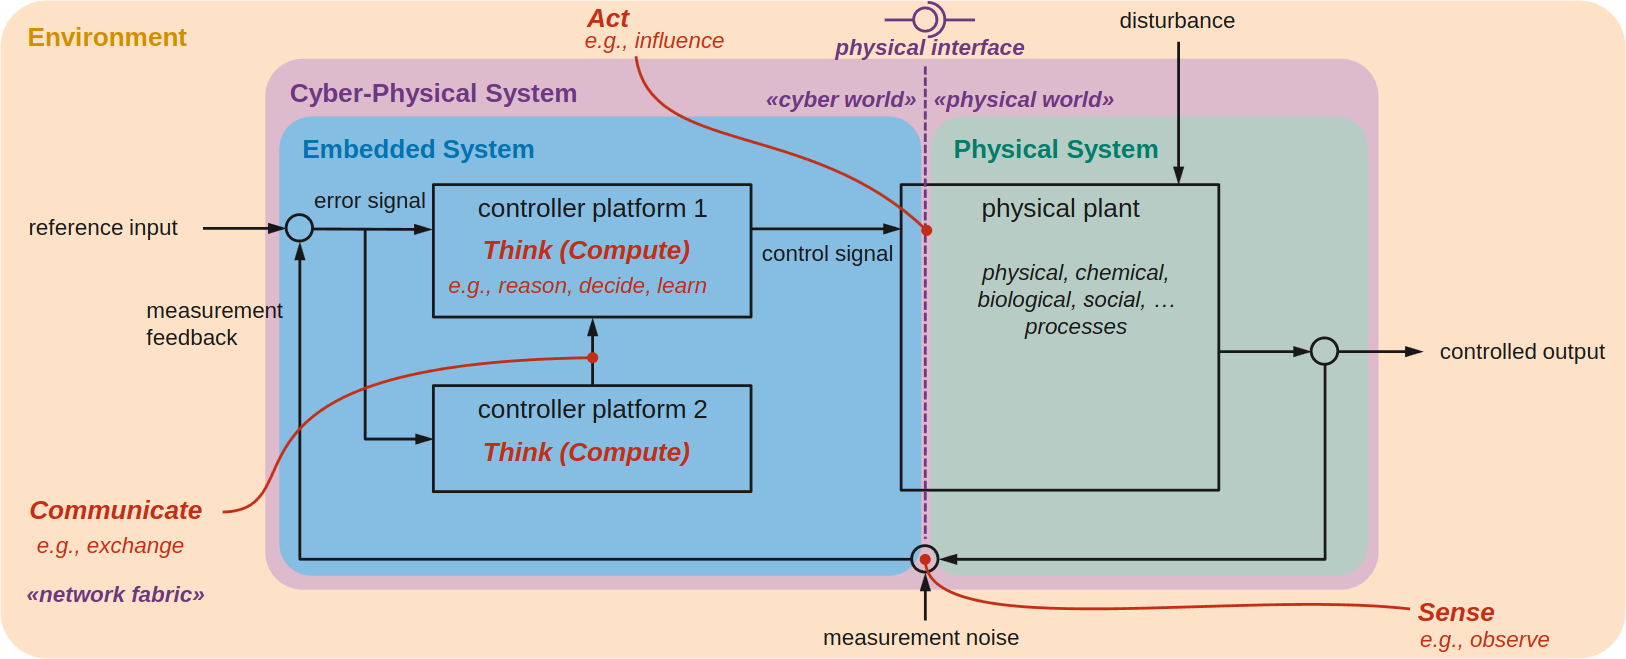
\includegraphics[width=\linewidth]{"Images/SenseThinkActCommunicate.png"}

\subsection{Schichtmodell}

\begin{center}
	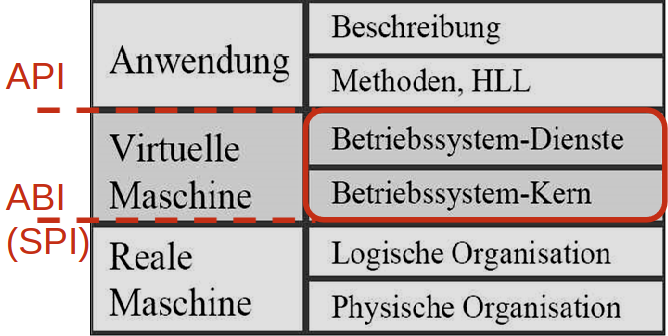
\includegraphics[width=.6\linewidth]{"Images/Schichtmodell.png"}
\end{center}

Das Betriebssystem im Schichtenmodell des Computersystems bietet der Anwendung API-Schnittstellen zur darunterliegenden realen Maschine und macht die Anwendung damit weitgehend unabhängig von der realen Maschine (CPU, Hardware, Peripherien,...).

\subsection{Mikrocontroller-Organisation}

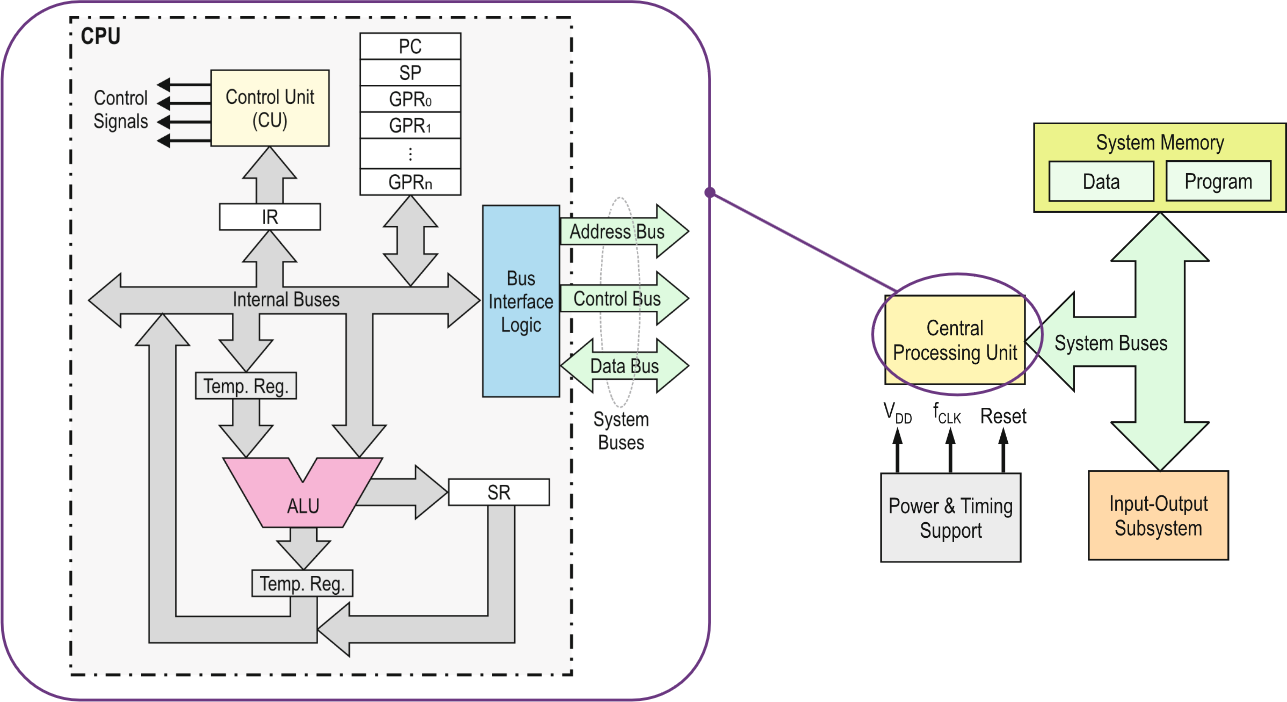
\includegraphics[width=\linewidth]{"Images/MikrocontrollerOrganisation.png"}
